\chapter{Configuration}
The graph visualization user interface is designed to be intuitive and easy to use. For most use cases the default configuration will offer a convenient GUI. However, more sophisticated occasions may require adapting the interface to specific needs. This is achieved by defining custom configuration files via JSON[\href{http://www.json.org}{json.org}]. The general configuration structure is shown in figure \ref{fig:configstruct}. The following sections will show how to work with the interface and create individual configurations.

\begin{figure} [h]
\centering
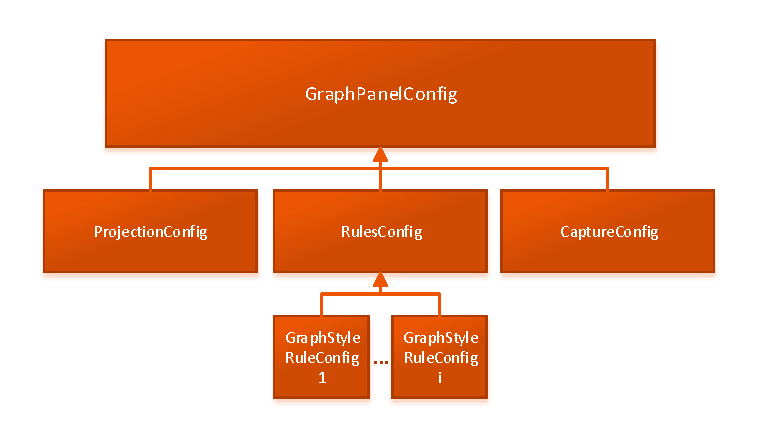
\includegraphics [scale=1] {images/configstruct.pdf}
\caption{Configuration Structure.}
\label{fig:configstruct}
\end{figure}


\section{GraphPanelConfig}
The GraphPanelConfig contains the most general configurable aspects as well as additional configuration objects, namely a \emph{ProjectionConfig}, a \emph{RulesConfig} and a \emph{CaptureConfig}. All configurable values and their descriptions are listed in \ref{tab:graphPanelConfigValues}.

\begin{table}[h]
\centering
\begin{tabular}[h]{|l|l|l|}\hline
	\textbf{Value} & \textbf{Type} & \textbf{Description}\\
	\hline
	Width & Integer & Width of the visualization window.\\
	\hline
	Height & Integer & Height of the visualization window.\\
	\hline
	Fullscreen & Boolean & If true the visualization window\\
	& & will be maximized on initialization.\\
	\hline
	StatPanelEnabled & Boolean & If true the visualization window\\
	& & will contain the StatPanel.\\
	\hline
	TextPanelEnabled & Boolean & If true the visualization window\\
	& & will contain the TextPanel.\\
	\hline
	TimetampFormat & String & Sets the used timestamp format.\\
	\hline
	RenderHQ & Boolean & Enables high-quality rendering.\\
	\hline
	RenderAA & Boolean & Enables anti-aliasing.\\
	\hline
	ZoomSpeed & Double & Zoom speed factor.\\
	\hline
	ScrollSpeed & Double & Scroll speed factor.\\
	\hline	
	ToolTipsEnabled & Boolean & If true tooltips will be enabled.\\
	\hline	
	DirectedEdgeArrowsEnabled & Boolean & If true directed edges will\\
	& & be rendered with arrow-heads.\\
	\hline
	NodeSize & Double & Default size of nodes.\\
	\hline
	NodeColor & String & Default color of nodes. All CSS color-\\
	& & keywords are available.\\
	& & See TODO CITE as reference.\\
	%http://www.w3schools.com/colors/colors_names.asp
	\hline
	EdgeSize & Double & Default size of edges.\\
	\hline
	Layouter & Enum & Layouter used to layout the graph.\\
	& & Possible values: none, auto, linlog.\\
	\hline
	AutoLayoutForce & Double & Force of the auto-layouter.\\
	\hline
	RulesConfig & JSON-Object & A rules config. See \ref{ss:rulesConfig}.\\
	\hline
	ProjectionConfig & JSON-Object & A Projection config. See \ref{ss:projectionConfig}.\\
	\hline
	CaptureConfig & JSON-Object & A capture config. See \ref{ss:captureConfig}.\\
	\hline
\end{tabular}
\caption{Configuration values of GraphPanelConfig.}
\label{tab:graphPanelConfigValues}
\end{table}

\subsection{RulesConfig}
\label{ss:rulesConfig}
The graph visualization allows to define so called \emph{GraphStyleRules} to modify the graph presentation in several ways. See \ref{s:graphStyleRules} for more details. In this section we focus on how to enable and configure said rules using the configuration. A RulesConfig holds multiple configurable \emph{GraphStyleRuleConfis}, each representing a single GraphStyleRule. Each GraphStyleRuleConfig will be identified by a key pointing to the rules class-path. Additionally, there are three shared configurable values for each rule: the \emph{name}, the \emph{enabled}-flag and the \emph{hidden}-flag. Furthermore, one may add additional parameters, which will be used by the respective rules. Note: The way these parameters will be treated is up to the given rule. See the following example \ref{config:exampleRuleConfig} for an actual RulesConfig definition. The first rule contains all possible configurable values and one additional parameter: \emph{Growth}. The NodeSizeByDegree class increases/decreases each nodes size by the growth-value whenever their degree is being incremented or decremented respectively. The second rule does not contain any values at all. However it will still be enabled.

\begin{figure} [h]
\begin{lstlisting}
"RulesConfig": {
	"dna.visualization.graph.rules.nodes.NodeSizeByDegree": {
		"Name": "defaultNodeSizeByDegree",
		"Growth": 0.3,
		"Enabled": true,
		"Hidden": false,
	},
	"dna.visualization.graph.rules.nodes.RandomNodeColor": {},
}
\end{lstlisting}
\caption{Example RuleConfig definition.}
\label{config:exampleRuleConfig}
\end{figure}

\begin{table}[h]
\centering
\begin{tabular}[h]{|l|l|l|}\hline
	\textbf{Value} & \textbf{Type} & \textbf{Description}\\
	\hline
	Name & String & Name of the rule.\\
	& & (If not set \emph{key} will be used as name.)\\
	\hline
	Enabled & Boolean & If set the rule is enabled.\\
	& & (If not set will be assumed as \emph{true}.)\\
	\hline
	Hidden & Boolean & If set the rule is hidden from the interface.\\
	& & (If not set will be assumed as \emph{false}.)\\
	\hline
	Parameter$_0$ & Parameter & First parameter of the respective rule.\\
	\hline
	Parameter$_1$ & Parameter & Second parameter of the respective rule.\\
	\hline
	... & ... & ...\\
	\hline	
	Parameter$_i$ & Parameter & i-th parameter of the respective rule.\\
	\hline
\end{tabular}
\caption{Configuration values of a GraphStyleRuleConfig.}
\label{tab:graphStyleRuleConfigValues}
\end{table}


\subsection{ProjectionConfig}
\label{ss:projectionConfig}
Since the graphstream library does not support three-dimensional coordinates, two simple projection mechanisms have been implemented to simulate 3D behaviour. In this mode the node weights are assumed as 3D coordinates. For all configurable values see \ref{tab:projectionConfigValues}.

\subsubsection{Vanishing Point Projection}
This projection mode uses a defined vanishing point and virtually \emph{shifts} all nodes towards the vanishing point. How far the nodes will be shifted depends on the respective $z$-coordinate. The further a point is away from the screen-plain ($z=0$) the further it will be shifted. The vanishing point coordinates, a scaling factor and logarithmic scaling can be configured in the ProjectionConfig. Note: If 3d-projection is enabled but vanishing point mode is disabled ortographic projection will be used instead.

\subsubsection{Ortographic Projection}
The ortographic projection uses a transformation matrix to project the three-dimensional nodes onto the two-dimensional screen-plain. The used matrix and a offset may be defined in the ProjectionConfig. Note: This this mode is only used if the vanishing point projection is disabled.

\begin{figure} [h]
\[
\left(
\begin{array}{c}
n_{x}^{'} \\
n_{y}^{'}
\end{array}
\right)
%
=
%
\left(
\begin{array}{ccc}
x_0 & y_0 & z_0 \\
x_1 & y_1 & z_1
\end{array}
\right)
\cdot
\left(
\begin{array}{c}
n_x  \\
n_y  \\
n_z
\end{array}
\right)
%
+
%
\left(
\begin{array}{c}
offset_x \\
offset_y
\end{array}
\right)
\]
\caption{Ortographic projection from node $n$ to two-dimensional node $n^{'}$.}
\label{math:orthographicProjection}
\end{figure}

\begin{table}[h]
\centering
\begin{tabular}[h]{|l|l|l|}\hline
	\textbf{Value} & \textbf{Type} & \textbf{Description}\\
	\hline
	Enabled & Boolean & If true 3d projection will be used.\\
	\hline
	UseVanishingPoint & Boolean & If true vanishing point will be used\\
	\hline
	VanishingPointLogScale & Boolean & If true the projection towards the\\
	& & VP will be scaled logarithmic.\\
	\hline
	VanishingPoint\textunderscore X & Double & $x$-coordinate of the VP.\\
	\hline
	VanishingPoint\textunderscore Y & Double & $y$-coordinate of the VP.\\
	\hline
	VanishingPoint\textunderscore Z & Double & $z$-coordinate of the VP.\\
	\hline
	VanishingPointScaling & Double & Weight of the projection scaling.\\
	\hline
	ScalingMatrixS0\textunderscore X & Double & $x_0$ value of the scaling matrix.\\
	& & For ortographic use only.\\
	\hline
	ScalingMatrixS0\textunderscore Y & Double & $y_0$ value of the scaling matrix.\\
	& & For ortographic use only.\\
	\hline
	ScalingMatrixS0\textunderscore Z & Double & $z_0$ value of the scaling matrix.\\
	& & For ortographic use only.\\
	\hline
	ScalingMatrixS1\textunderscore X & Double & $x_1$ value of the scaling matrix.\\
	& & For ortographic use only.\\
	\hline
	ScalingMatrixS1\textunderscore Y & Double & $y_1$ value of the scaling matrix.\\
	& & For ortographic use only.\\
	\hline
	ScalingMatrixS1\textunderscore Z & Double & $z_1$ value of the scaling matrix.\\
	& & For ortographic use only.\\
	\hline
	OffsetVector\textunderscore X & Double & $x$-value of the offset vector.\\
	& & For ortographic use only.\\
	\hline
	OffsetVector\textunderscore Y & Double & $y$-value of the offset vector.\\
	& & For ortographic use only.\\
	\hline
\end{tabular}
\caption{Configuration values of a ProjectionConfig.}
\label{tab:projectionConfigValues}
\end{table}

\subsection{CaptureConfig}
\label{ss:captureConfig}
TODO

\begin{table}[h]
\centering
\begin{tabular}[h]{|l|l|l|}\hline
	\textbf{Value} & \textbf{Type} & \textbf{Description}\\
	\hline
	CaptureArea & Enum & Default area to be recorded.\\
	& & Possible values: content, graph, full\\
	\hline
	VideoDir & String & Destination directory for captured videos.\\
	\hline
	VideoSuffix & String & Suffix of video files.\\
	\hline
	VideoFilename & String & Filename of captured video files. If set as\\
	& & "null" names will be derived from the graph-\\
	& & panel name and (real-time) timestamp.\\
	\hline
	VideoMaximumLength & Integer & Maximum length of videos in seconds.\\
	\hline
	VideoRecordFPS & Integer & Frames per second of the resultin video.\\
	\hline
	VideoAutoRecrod & Boolean & If set video recording will automatically\\
	& & start upon initialization.\\
	\hline
	ScreenshotDir & String & Destination directory for screenshots.\\
	\hline
	ScreenshotFormat & String & Screenshot format (png, jpg...).\\
	\hline
	ScreenshotStabilityThreshold & Double & Stability threshold of the layouter when\\
	& & taking screenshots waiting for stability.\\
	\hline
	ScreenshotStabilityTimeout & Long & Stability timeout for taking screenshots\\
	& & waiting for stability in ms.\\
	\hline
	ScreenshotForegroundDelay & Long & Artificial delay when taking screenshots to\\
	& & let the machine move the panel to foreground.\\
	\hline
\end{tabular}
\caption{Configuration values of CaptureConfig.}
\label{tab:captureConfigValues}
\end{table}

\section{Default-Configuration file}
TODO

\section{Building own configuration files}
TODO